\subsection*{Flujo de efectivo}
\addcontentsline{toc}{subsection}{Flujo de efectivo}

Mediante el flujo de efectivo se puede determinar la capacidad de la compañía para generar dinero y cumplir con sus compromisos financieros, realizar inversiones y llevar a cabo otros procesos de expansión.

Existen tres tipos de flujos de caja que contribuyen a calcular el flujo neto:

\begin{itemize}
	\item \textbf{Flujo de caja de operación:} Se obtiene a partir de la utilidad presentada en el estado de resultados. Incluye elementos como la depreciación, la amortización, los intereses de la deuda y los impuestos sobre la renta.
	
	\item \textbf{Flujo de caja de inversión:} Agrupa todas las inversiones necesarias para el correcto funcionamiento de la empresa, considerando tanto las inversiones en activos tangibles como en activos intangibles.
	
	\item \textbf{Flujo de caja de financiamiento:} Refleja el dinero que ingresa a través de inversionistas, así como otros movimientos relacionados con la financiación de la empresa.
\end{itemize}

La suma de estos tres tipos de flujos de caja da como resultado la cantidad de efectivo que la empresa generó durante el año analizado.

\begin{table}[H]
	\centering
	\caption[{Flujo de efectivo}]{\centering Flujo de efectivo. \textit{Fuente:} Autores.}
	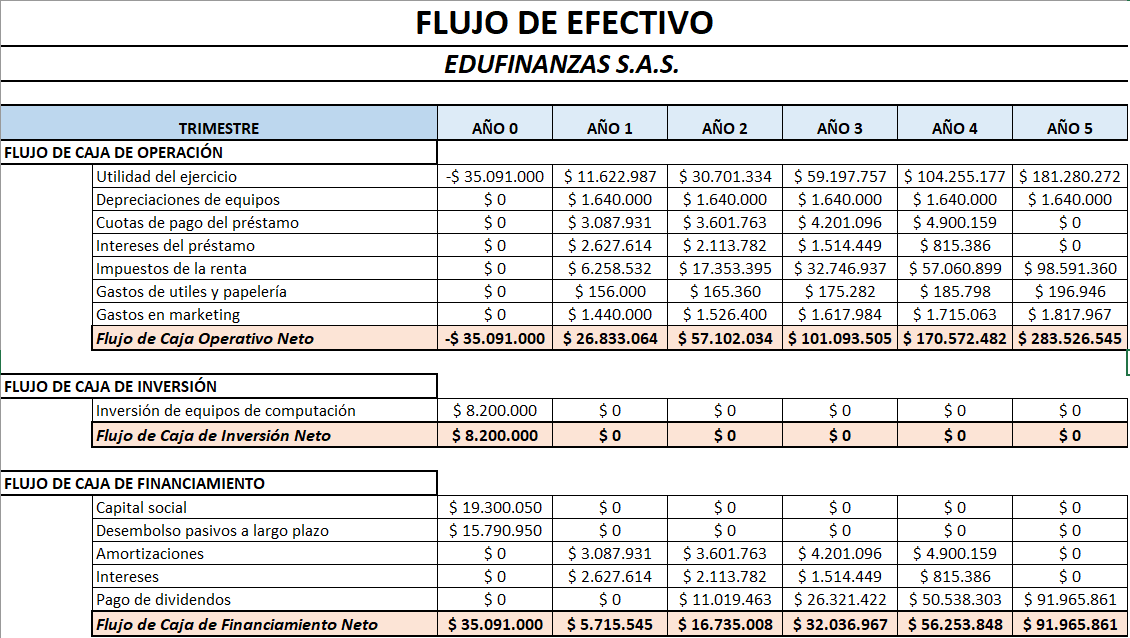
\includegraphics[width=15cm]{Imagenes/FlujoEfectivo.png}
	\label{FlujoEfectivo}
\end{table}